\subsection{Audio Out Port}

The \systemName~includes an audio port that is connected to the HDMI
Transmitter chip on the \DEBoard~board. The default setting for the 
sample rate provided by the audio port is 
32K samples/sec.  The port provides audio output functionality.  
The audio port includes two FIFOs that are used to hold outgoing data.
Outgoing data is held in the left- and right-channel {\it Write} FIFOs. Both FIFOs have a maximum 
depth of 128 32-bit words.

The audio port's programming interface consists of four 32-bit registers, as illustrated in 
Figure \ref{fig:audio_port}.  The {\it Control} register, which has the address 
{\sf 0xFF203040}, is readable to provide status information and writable to make control
settings. 
Bit {\it WE} gives an interrupt enable capability for outgoing data. Setting this bit to 
1 allows the audio core to generate an interrupt when either of the {\it Write} FIFOs are
less that 25\% full. The bit {\it WI} will be set to 1 to indicate that the interrupt 
is pending, and it can be cleared by filling the {\it Write} FIFOs until both 
are more than 25\% full.  The bit {\it CW} in Figure \ref{fig:audio_port} can 
be set to 1 to clear the {\it Write} FIFOs. The clear function 
remains active until the corresponding bit is set back to 0.

\begin{figure}[h!]
   \begin{center}
       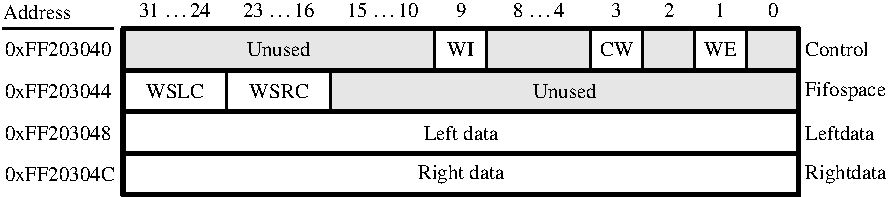
\includegraphics{../../../common/figs/Media_FPGA_Audio_Address_Map_Out_Only.pdf}
   \end{center}
   \caption{Audio port registers.}
	\label{fig:audio_port}
\end{figure}

The read-only {\it Fifospace} register in Figure \ref{fig:audio_port} contains four 8-bit fields.
The fields {\it WSRC} and {\it WSLC} give 
the number of words currently available (that is, {\it unused}) for storing data in the right 
and left audio-out FIFOs. When all FIFOs in the audio port are cleared, the values provided 
in the {\it Fifospace} register are {\it WSRC} $=$ {\it WSLC} $=$ 128.

The {\it Leftdata} and {\it Rightdata} registers are writable
for audio out. When data is written into these registers it is loaded into the {\it
Write} FIFOs.

Note that the HDMI audio requires the HDMI video-out signals 
\textit{HDMI\_TX\_HS} (Horizontal Synchronization) and 
\textit{HDMI\_TX\_VS} (Vertical Synchronization) to be connected.

